% Nallino, Part I p. 318: the triangle of the qiblah, redrawn from the print: the meridian CB of Mekkah, the arc CA
% perpendicular to it, the great circle AB from the city A to Mekkah B, and the double mark of the angle BAC.
% Measured on the scan (_intake/latin/tools/fig318).
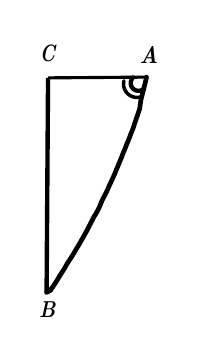
\begin{tikzpicture}[x=0.9921pt,y=-0.9921pt,line cap=butt,every node/.style={font=\fontsize{11}{11}\bfseries\itshape\selectfont,inner sep=0pt}]
\useasboundingbox (0,0) rectangle (58.00,103.00);
\draw[line width=1.13pt] (7.42,18.28) -- (43.29,18.01);  % the arc CA, perpendicular to the meridian, from C to A
\draw[line width=1.58pt] (7.42,18.28) -- (6.89,96.42);  % the meridian CB of Mekkah, from C to B (printed heavier)
\draw[line width=1.69pt,line join=round,line cap=round] (43.29,18.01) -- (43.09,18.93) -- (42.87,19.84) -- (42.65,20.75) -- (42.43,21.66) -- (42.20,22.57) -- (41.97,23.48) -- (41.74,24.39) -- (41.50,25.29) -- (41.27,26.20) -- (41.14,27.02) -- (41.04,27.77) -- (40.95,28.43) -- (40.86,29.01) -- (40.80,29.51) -- (40.63,30.01) -- (40.47,30.51) -- (40.29,31.01) -- (40.14,31.51) -- (39.96,32.01) -- (39.80,32.51) -- (39.61,33.01) -- (39.44,33.51) -- (39.26,34.01) -- (39.09,34.51) -- (38.91,35.01) -- (38.76,35.51) -- (38.60,36.01) -- (38.43,36.51) -- (38.25,37.01) -- (38.06,37.51) -- (37.84,38.01) -- (37.64,38.51) -- (37.45,39.01) -- (37.27,39.51) -- (37.08,40.01) -- (36.88,40.51) -- (36.68,41.01) -- (36.48,41.51) -- (36.26,42.01) -- (36.06,42.51) -- (35.88,43.01) -- (35.68,43.51) -- (35.48,44.01) -- (35.28,44.51) -- (35.06,45.01) -- (34.84,45.51) -- (34.64,46.01) -- (34.45,46.51) -- (34.27,47.01) -- (34.06,47.51) -- (33.85,48.01) -- (33.64,48.51) -- (33.44,49.01) -- (33.22,49.51) -- (33.03,50.01) -- (32.83,50.51) -- (32.61,51.01) -- (32.40,51.51) -- (32.18,52.01) -- (31.99,52.51) -- (31.78,53.01) -- (31.58,53.51) -- (31.35,54.01) -- (31.14,54.51) -- (30.91,55.01) -- (30.69,55.51) -- (30.44,56.01) -- (30.21,56.51) -- (29.98,57.01) -- (29.74,57.51) -- (29.52,58.01) -- (29.31,58.51) -- (29.08,59.01) -- (28.86,59.51) -- (28.62,60.01) -- (28.35,60.51) -- (28.09,61.01) -- (27.84,61.51) -- (27.56,62.01) -- (27.31,62.51) -- (27.08,63.01) -- (26.86,63.51) -- (26.66,64.01) -- (26.46,64.51) -- (26.25,65.01) -- (26.04,65.51) -- (25.81,66.01) -- (25.54,66.51) -- (25.29,67.01) -- (25.00,67.51) -- (24.72,68.01) -- (24.37,68.51) -- (24.08,69.01) -- (23.82,69.51) -- (23.55,70.01) -- (23.29,70.51) -- (23.06,71.01) -- (22.80,71.51) -- (22.53,72.01) -- (22.27,72.51) -- (22.00,73.01) -- (21.76,73.51) -- (21.52,74.01) -- (21.24,74.51) -- (20.96,75.01) -- (20.67,75.51) -- (20.40,76.01) -- (20.10,76.51) -- (19.81,77.01) -- (19.54,77.51) -- (19.28,78.01) -- (18.98,78.51) -- (18.69,79.01) -- (18.39,79.51) -- (18.09,80.01) -- (17.78,80.51) -- (17.48,81.01) -- (17.18,81.51) -- (16.89,82.01) -- (16.59,82.51) -- (16.29,83.01) -- (15.99,83.51) -- (15.68,84.01) -- (15.34,84.51) -- (15.00,85.01) -- (14.67,85.51) -- (14.36,86.01) -- (14.06,86.51) -- (13.80,87.01) -- (13.50,87.51) -- (13.20,88.01) -- (12.88,88.51) -- (12.56,89.01) -- (12.21,89.51) -- (11.91,90.01) -- (11.61,90.51) -- (11.31,91.01) -- (11.01,91.51) -- (10.72,92.01) -- (10.41,92.51) -- (10.08,93.01) -- (9.74,93.51) -- (9.42,94.01) -- (9.12,94.51) -- (8.55,95.09) -- (8.60,95.51) -- (6.89,96.42);  % the great circle AB from the city A to Mekkah B, traced along its centre line
\draw[line width=1.55pt,line join=round,line cap=round] (42.02,22.45) -- (41.71,22.65) -- (41.37,22.80) -- (41.02,22.91) -- (40.66,22.98) -- (40.29,23.00) -- (39.92,22.96) -- (39.56,22.88) -- (39.21,22.76) -- (38.88,22.58) -- (38.58,22.37) -- (38.31,22.12) -- (38.07,21.84) -- (37.87,21.52) -- (37.72,21.19) -- (37.61,20.83) -- (37.54,20.47) -- (37.53,20.10) -- (37.57,19.73) -- (37.65,19.37) -- (37.78,19.02) -- (37.95,18.69) -- (38.17,18.39) -- (38.42,18.12);  % the inner arc of the mark of the angle at A
\draw[line width=1.25pt,line join=round,line cap=round] (41.67,25.04) -- (41.23,25.20) -- (40.78,25.31) -- (40.32,25.38) -- (39.85,25.41) -- (39.39,25.39) -- (38.92,25.33) -- (38.47,25.22) -- (38.03,25.07) -- (37.60,24.88) -- (37.19,24.65) -- (36.81,24.38) -- (36.46,24.08) -- (36.13,23.74) -- (35.84,23.38) -- (35.59,22.99) -- (35.37,22.57) -- (35.20,22.14) -- (35.06,21.69) -- (34.97,21.23) -- (34.93,20.77) -- (34.92,20.30) -- (34.97,19.84) -- (35.05,19.38);  % the outer arc of the mark of the angle at A
\node at (7.22,9.48) {\normalfont\fontsize{11}{11}\bfseries\itshape\selectfont \resizebox{5.51pt}{5.86pt}{C}};
\node at (44.17,10.20) {\normalfont\fontsize{11}{11}\bfseries\itshape\selectfont \resizebox{6.70pt}{5.93pt}{A}};
\node at (7.13,102.72) {\normalfont\fontsize{11}{11}\bfseries\itshape\selectfont \resizebox{5.91pt}{5.70pt}{B}};
\end{tikzpicture}
